% !TeX root = ../main.tex
% Add the above to each chapter to make compiling the PDF easier in some editors.

\chapter{Methodology / AlgoFuzz}\label{chapter:methodology}
The primary objective of this research is to design and develop AlgoFuzz, a fuzzer tailored for Algorand smart contracts.
This chapter will detail the methodology employed, breaking down each step and rationale.
By clarifying our considerations and assumptions behind specific decisions we aim to allow future researchers or developers to build upon our work.

\section{Fuzzing Approach}

\subsection*{Input Generation}
When making an Application call on Algorand, the data that is passed can be completely arbitrary.
The smart contract developer can decide on the format of the data and how it should be interpreted.
This means that the general approach of generating random inputs, could be suitable for such cases.
However, generating inputs in a completely random fashion is not very effective because the probability of generating a valid input is very low.
The vast majority of inputs will be rejected by the application.
For this reason, we consider for our fuzzer only contracts that adhere to the official \ac{ABI} conventions.
What we generate will be aware of the input structure of the contract.
This provided us with the different functions that are available in the smart contract and the types of the arguments that they take.
From this information, comes the first part of the fuzzed input, the second part is the account that is used to call the smart contract.
Our fuzzing input would then be the following tuple: \texttt{(function, arguments, account)}.
To generate the inputs for our fuzzer we will be using a mutation-based approach.
This approach is a good starting point since it is simple to implement, has been shown to be effective in previous works and it can be extended in the future to include more sophisticated techniques.
For now, the inputs will be seeded with a minimal value according to their type, such as an empty string.
In the future, it would be interesting to have the user specify some valid seed values for the different arguments.

\subsection*{Fault Detection}
Based on our research on Algorand smart contracts, we decided to develop a property-based fuzzer for Algorand.
As discussed in \ref{section:algorand-smartcontracts}, detecting errors that commonly happen in Algorand smart contracts can be better done by a static analyzer.
For the evaluation of the input, the user can define properties that should hold for the contract.
Alternatively, they can run the fuzzing in \textit{Assertion Mode} which will check for all the possible assertion failures on application calls.
The properties that the user can define will be dependent on the state of the contract.
With the state, the user can define arbitrary invariants which should always hold (return \texttt{true}).
Unfortunately due to limitations of the current version of Algorand nodes we will only be able to retrieve the global and local state of an application.
The methods that manipulate the box state of the application are currently not implemented for \texttt{dryrun} calls.
Dryrun calls are used to simulate the execution of a transaction without actually executing it.
They are important for our fuzzer since they allow us to retrieve the coverage information of an application call, which is used as a guiding metric for the fuzzing process (discussed in \ref{section:drivers}).

\subsection*{Granularity of Analysis}
For the fuzzer to be as general as possible, we decided to make it work with any contract written with \ac{TEAL} without considering the higher level tool (such as PyTeal or TEALScript) used to write the contract.
Although the fuzzer will have access to the \ac{TEAL} code of the contract and the \ac{ABI}, it will not be able to leverage white box fuzzing techniques.
We decided this was outside the scope of this research due to the complexity of implementing such a fuzzer.
Such a fuzzer would need to be able to parse the \ac{TEAL} code and understand the semantics of the different opcodes.

For our project, we decided to focus on a grey box approach.
The inputs generated by the fuzzer will be guided by different metrics that we gather during the process.
When an input covers more code than previous inputs or produces a new state transition, it is considered interesting.
Code coverage is the most common metric used to guide the fuzzing process.
An advantage of using coverage is that it gives us a metric that can be used to compare our fuzzer to other fuzzers.
Since our fuzzer relies on property tests on the state of the contract to detect bugs, it makes sense to have a fuzzer which optimizes for generating inputs that produce different states.

\subsection*{Stopping Condition}
The stopping condition of the fuzzer can be configured in multiple ways.
Similar to Algorithm \ref{alg:fuzz}, the fuzzer can be configured to run for a maximum amount of time.
Alternatively, the maximum number of calls executed by the fuzzer can be specified.
In both cases, the fuzzer can be stopped prematurely if an input breaks a property test or an assertion failure is detected.
This is slightly different from the approach most fuzzers take, where the fuzzer runs for the whole duration and gathers all possible bugs during the process.
The reason for this is that we want to see if there is a bug in the contract, opposed to how many bugs there are.
Smart contracts are usually small programs \cite{gao_checking_2021}, so they are not expected to have many bugs.

\section{AlgoFuzz Design}

\subsection*{Execution Environment}
\paragraph*{Contract.} The smart contracts being fuzzed will be deployed on a local Algorand network. This network usually comes with the official AlgoKit CLI tool \cite{noauthor_algokit_nodate}. The setup for such a network is straightforward and can be done with a single command. The local network starts three docker containers to simulate the Algorand blockchain with a \acs{REST} \acs{API} for users to interact with the local network outside the container.

We also looked at different interpreters for \ac{TEAL} that simulate the \ac{AVM} such as teal-interpreter \cite{noauthor_hone-labsteal-interpreter_nodate} and the AlgoBuilder Runtime \cite{noauthor_algo-builderruntime_nodate}.
Both these projects can be import as NPM packages to be used in JavaScript projects.
We decided against using these tools for the following reasons:
\begin{itemize}
    \item They are not official tools and are not maintained by the Algorand Foundation.
    \item They are not as well documented as the official tools.
    \item Executing the smart contracts on the local network is most similar to how they would be executed on the Algorand network.
    \item teal-interpreter has had no commits in more than one year, supports only up to \ac{TEAL} version 5 (current version is 8) and does not support all opcodes.
\end{itemize}

\paragraph*{Fuzzer.} The fuzzer is implemented \acs{API} of the local network.
We decided to use Python since we also wanted to use PyTeal to write our own Algorand contracts.
This way we can easily write test suites for our contracts.
Fuzzers usually rely on generating a large amount of inputs and therefore need a very performant language.
Although Python is not the fastest language, we expected most of the time to be spent on the \acs{API} calls to the local network.

\subsection*{Limitations}
Despite the advantages, using the technologies and approaches that we have chosen comes with some limitations.
The first one being that the performance of our fuzzer will be limited by the performance of the local network.
The local network is relatively slow since it simulates all Algorand blockchain operations, such as adding and verifying blocks.
Due to this, we also need to fund the accounts that we use for the fuzzing process which requires a transaction from a dispenser account to the account being funded.
Parallelizing the fuzzing process would also not work.
Even though the local network can take multiple transactions at the same time, it will only execute them sequentially.
Aside from this, making requests back and forth to the local network is slower than having an interpreter in the same process.
Also, to retrieve the coverage information of an application call, we need to make two requests to the local network (\texttt{dryrun} and the actual transaction).

The other limitations are functional in nature.
As mentioned we cannot access the box state of the application, because it is not supported by the \texttt{dryrun} call.
This means that contracts that rely on dynamic storage are not supported or impractical to replicate for our fuzzer.

Our tool will initially not be supporting all argument types, from the \ac{ABI}, but it will be supporting the most common ones.
The most important types left out will be:
\begin{itemize}
    \item \texttt{address}: This type is used to represent an address on the Algorand network.
          Giving random addresses in this case is not a good idea since the address is a 58 byte array that is encoded in base32.
          This means that the probability of generating a valid address is very low. For this reason, we decided to leave this type out of the initial implementation.
    \item \texttt{reference types}: Aside from the account reference type, all other reference types will not be supported since they are difficult to generate.
          For example, working with assets requires the user to opt-in to the asset as well as the application being fuzzed.
          Since this feature is not currently supported also generating an asset reference is not possible.
\end{itemize}

Another limitation of our tool is that it expects opt-in calls to be empty.
In some Algorand contracts, opt-in calls may be connected to a certain function call that requires specific arguments.
Currently, it is not possible to infer from the \ac{ABI} of the contract with which function an opt-in call is connected to.
Therefore, we decided to leave this feature out of the initial implementation and we opt in all required accounts with empty application calls.
Similarly to the opt-in calls, all other special calls are not executed by our tool.
The fuzzer only executes noop applications calls.
In the future, we could extend our tool to also randomly execute special calls.

\subsection*{Architecture}
The architecture of our solution is shown in Figure \ref{fig:algofuzz-architecture}.
We extended the generic architecture in Figure \ref{fig:generic-fuzzer-architecture} by adding multiple ways to guide the fuzzing process through our different drivers which are passed on to the \texttt{ContractFuzzer}.
Aside from that, we use mutations for our input generation. Since we have to support multiple different data types, the base Mutator is shown as an \texttt{Interface} which will be implemented by specific Mutator classes.
To handle operations connected to the local network, we created \texttt{FuzzAppClient} which is a wrapper around the \texttt{ApplicationClient} from the AlgoKit.
It encapsulates all the logic for making calls to the local network and retrieving the results.
In Section \ref{section:implementation} we will go over the implementation details of the different modules.

\begin{figure}[htbp]
    \centering
    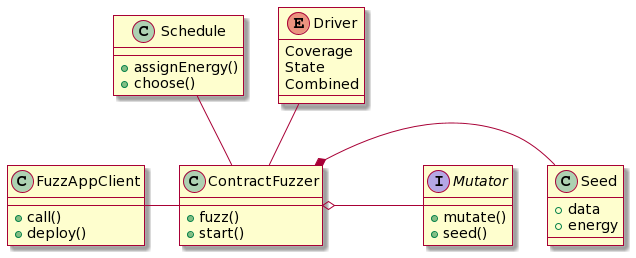
\includegraphics[width=0.85\textwidth]{figures/arc.png}
    \caption{Architecture of AlgoFuzz}\label{fig:algofuzz-architecture}
\end{figure}

\section{Implementation} \label{section:implementation}

\subsection*{FuzzAppClient}

\begin{figure}[htbp]
    \centering
    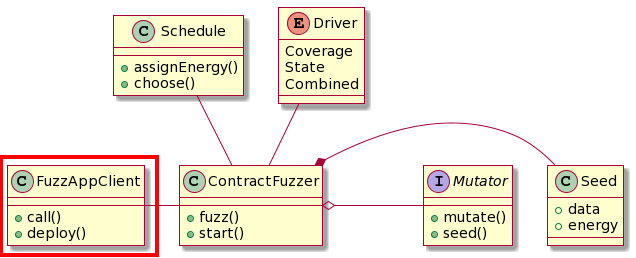
\includegraphics[width=0.85\textwidth]{figures/arc-client.png}
    \caption{AlgoFuzz architecture with FuzzAppClient highlighted.}\label{fig:architecture-client}
\end{figure}

The first thing we had to do was find a way to interact with the local network.
In the beginning, we used the Algorand Python \ac{SDK} \cite{noauthor_algorand_nodate-5} directly to make calls to the local network.
This worked fine for the most part, but it required us to write a lot of code for generic operations when we wanted to interact with an application.
For example, to make an application call we had to create a transaction, sign it, send it to the network, wait for the transaction to be confirmed, and then retrieve the result.
Later we found out that Algokit provides a standard client for applications, called \texttt{ApplicationClient}, which encapsulates most of these operations, and it also works with \ac{TEAL} contracts.
To make the client more suitable for our use case, we created a wrapper around it called \texttt{FuzzAppClient}.
This wrapper adds the following functionality:
\begin{itemize}
    \item Gathering coverage information from every application call. This is done by making a \texttt{dryrun} call before the actual application call.
    \item Preparing application call arguments such as payments, by creating the corresponding transactions.
    \item Changing the account that is used to make the application call.
    \item Opting in to the application all the accounts that are used for the fuzzing process.
    \item Disassembling the \ac{TEAL} code of the contract and retrieving the total number of lines.
          %\item Reporting assertion failures and differentiating them from other errors.
\end{itemize}


\subsection*{Mutators} \label{section:mutators}
In this section we will go through the mutators and the heuristics that we implemented for our fuzzer.
A mutator has two important methods:
\begin{itemize}
    \item \texttt{mutate}: This method takes an input and mutates it.
          Internally, a mutator may have multiple mutation strategies that it uses to mutate the input.
    \item \texttt{seed}: This method seeds the input with a value.
          Currently, we have chosen simple initial values for all different types.
\end{itemize}


\begin{figure}[htbp]
    \centering
    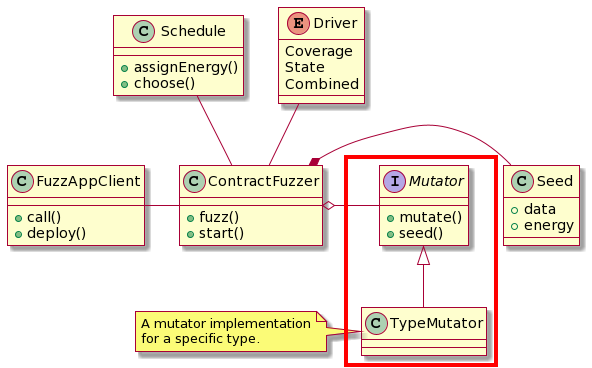
\includegraphics[width=0.85\textwidth]{figures/arc-mutator-r.png}
    \caption{AlgoFuzz architecture with mutator highlighted.}\label{fig:architecture-mutator}
\end{figure}

\paragraph{Boolean.} This mutator generates random boolean values. The values are all seeded with \texttt{False}.
The mutation strategy is simply to flip the value of the boolean.

\paragraph{Uint, Ufixed and Byte.}
The Uint mutator generates random unsigned integer values. It is initialized with the size of the integer, from 8 to 256 bits. The seed value used is 0, since it is the smallest possible value and also a commonly used value. The mutation function chooses randomly from the following mutation strategies are used:
\begin{itemize}
    \item add - Adds a random value without overflowing.
    \item subtract - Subtracts a random value without underflowing.
    \item multiply - Multiplies the value with a random value without overflowing.
    \item divide - Divides the value with a random value without underflowing.
    \item random bit flip - Flips a random bit in the value.
    \item bitwise and - Performs a bitwise and with a random value.
    \item bitwise or - Performs a bitwise or with a random value.
    \item bitwise xor - Performs a bitwise xor with a random value.
\end{itemize}
The effectiveness of these strategies in fuzzing has been shown in previous works and we expect them to be effective in our case as well.

Ufixed and Byte mutators are special cases of the Uint mutator. The Ufixed mutator is initialized with the size of the integer part and the size of the fractional part. When mutating the value is first converted to an unsigned integer, mutated and then converted back to a fixed point number by dividing it with the fractional part size. The Byte mutator is an alias for the Uint mutator with a size of 8 bits.

\paragraph{String, Array Dynamic and Array Static.}
The String mutator and the dynamic length Array mutator work similarly. They are seeded with an empty string or array. Then one of the following mutation strategies is randomly chosen:
\begin{itemize}
    \item add - Adds a random value to the string or array at a random position.
    \item remove - Removes a random value to the string or array at a random position if the string or array is not empty.
    \item flip - Replaces a random value in the string or array with a random value.
\end{itemize}

The difference between the two is that the array mutator also initializes a mutator for the type of the array.
This mutator is used to generate the random values to be added by mutating the seed or when flipping a value by mutating the value at the corresponding position.
The static length Array mutator is identical to the dynamic length Array mutator, except that it can only use the flip element mutation strategy.
Therefore, not changing the size of the array.

\paragraph{Tuple.}
For the tuple mutator, we initialize a mutator according to each type in the tuple.
When mutating the tuple, we mutate each element of the tuple with the corresponding mutator.
The seed value is a tuple of the seed values of the mutators.

\paragraph{Account.}
The account mutator is needed not only to generate an account as an argument for an application call but also to generate the account which will be executing the call.
This mutator is initialized with a list of funded accounts.
Each account having a balance of 200 Algos.
The seed value is the first account in the list.
When the mutation method is called, we either return the current account passed to the mutator or we choose a random account from the list of funded accounts.
This means that there is a 66\% chance that the account will stay the same and a 33\% chance that it will change.
The reason for this is that we do not want the account to change too often.
This insures that some calls will be executed from the current before switching to another account.

\paragraph{Payment.}
The payment mutator is used to generate payment objects for method calls which require a payment.
The payment object contains only the amount of Algos to be transferred.
These objects are then transformed into a payment transaction and grouped with the application call.
The recipient of the payment is always the account of the application being fuzzed.
Since we are using a local network, we cannot send arbitrary amounts of Algos as there is a limit on the amount of Algos available.
The amount of Algos send will just be a random value between 0 and 100 Algos, which is around the average transaction on Algorand.
In the future this could be a configurable value for the fuzzer.
When one of the accounts has less than 200 Algos, we fund the account with an additional 1 million Algos.
This way our transaction does not fail due to insufficient funds.


\paragraph{Method Mutator.}
The method mutator is initialized by passing an \ac{ABI} method.
Similar to the tuple mutator, we initialize a mutator for each argument of the method.
The mutating strategy differs from the tuple mutator.
We first generate a random number from 1 to the number of arguments of the method which will be the number of arguments that we mutate.
Then we use this number to sample the indices of the arguments that we will mutate.
For the sampled indices, we mutate the argument with the respective mutator.


\subsection*{Contract Fuzzer}
For most smart contracts, the code of different methods is relatively independent to each other.
Meaning the vast majority of methods are small, self-contained, and they rarely call common subroutines.
From this point of view each method of the contract can be seen as a separate program.
This means that we can fuzz each method separately and then combine the results.
We call this approach \textit{partial fuzzing} (similar to a partial derivative in math). The second approach that we implemented is \textit{total fuzzing}.
In this case, the fuzzer contains all necessary fuzzing parameters to fuzz the entire contract.
In Figure \ref{fig:architecture-fuzzers} we can see the updated architecture with the two types of fuzzers.

\begin{figure}[htbp]
    \centering
    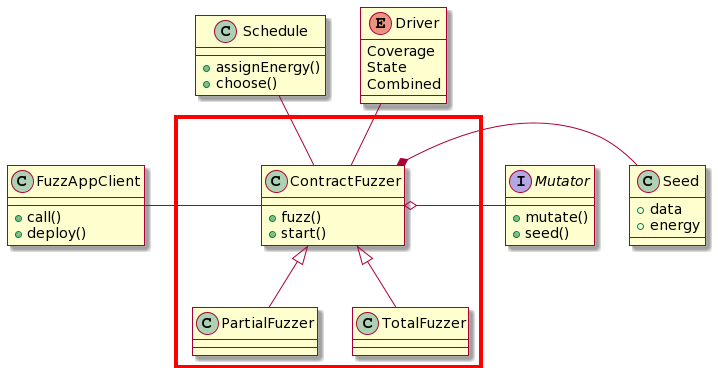
\includegraphics[width=0.85\textwidth]{figures/arc-fuzzers-r.png}
    \caption{AlgoFuzz architecture with two types of fuzzers.}\label{fig:architecture-fuzzers}
\end{figure}

\paragraph{Partial Fuzzer.} During fuzzing, the partial fuzzer creates only one application and a separate fuzzer for each method.
These \textit{method fuzzers} each have their own population of interesting inputs, power schedules, seeds, and other fuzzing parameters.
The population of inputs in this case being a list of tuples of the form \texttt{(arguments, account)}.
On each iteration the partial fuzzer randomly chooses a method and runs the corresponding method fuzzer.
All methods have the same probability of being chosen regardless of the amount interesting inputs are found for them.
Although this approach seems naive, it has been shown to be reasonably effective in practice from our experiments.
The main advantage of this approach is that it is very easy to implement and it generates new inputs faster.
The performance gain comes from the fact that the schedulers of the different method fuzzers have fewer inputs to choose from.
Another subtle advantage of the partial fuzzer is that methods which do not produce any interesting input during the seeding stage will not be completely ignored in the future fuzzing process.

\paragraph{Total Fuzzer.} Different from the method fuzzers in the partial fuzzer, the population of inputs is a list of tuples of the form \texttt{(function, arguments, account)}.
This means that functions that produce more interesting inputs will be fuzzed more often which is the main advantage compared to the partial fuzzer.
The main disadvantage is that methods which do not produce any interesting input during the seeding stage will be consequently completely ignored.
To avoid this problem, we introduced a breakout mechanism through a coefficient passed to the constructor of the fuzzer.
This coefficient is used to determine the probability of uniformly randomly choosing one of the seeds and producing a new input by mutating it.
Since we create a seed for each function, there is a chance that the seed of a function that does not produce any interesting inputs is chosen.
We applied this breakout mechanism to the method fuzzers as well.



\subsection*{Drivers}\label{section:drivers}
Most fuzzers use different metrics to determine which inputs are interesting and which are not.
We call these metrics the \textit{drivers} of the fuzzer.
In this section, we will discuss the different drivers that we chose for our fuzzer.


\begin{figure}[htbp]
    \centering
    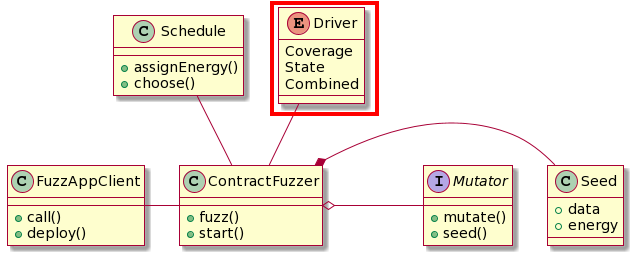
\includegraphics[width=0.85\textwidth]{figures/arc-driver.png}
    \caption{AlgoFuzz architecture with driver highlighted.}\label{fig:architecture-driver}
\end{figure}

\paragraph{Coverage Driver.}
As mentioned most fuzzers use some sort of coverage information to guide the fuzzing process.
This is also the case for our fuzzer.
The coverage information is retrieved by running the application call in \texttt{dryrun} mode.
What we retrieve from the \texttt{dryrun} call only tells us which lines of the code were executed.
Although we can use this information to detect promising inputs, applying better heuristics, such as directed fuzzing, is not possible.
The coverage information of a call is processed by creating a set of all the lines that were executed.
This set is called a coverage path.
If an input produces a new coverage path, it is considered interesting.

\paragraph{State Driver.}
Since our fuzzer relies on property tests on the state of the contract to detect bugs, it makes sense to have a fuzzer which optimizes for generating inputs that produce different states.
To use the state as a driver, we retrieve the global state of the application and the local states of the accounts in the account mutator.
We then hash this information to create a unique identifier for the state and not store the entire state.
This is necessary since the state can be very large and storing it for each input could be very expensive.
One way of using this information to identify interesting inputs is by detecting if it produced a new state.
This works fine, but we decided to consider transitions between states as interesting inputs.
The reason for this is that in the future these transitions can be used to find the input sequence the produces a bug.
This can be done by going through the transition graph and finding the shortest path between the initial state and the state that produces the bug.
In Echidna this process is called \textit{shrinking}.
The shrinking process is not implemented in our fuzzer, but it is a possible extension.

\paragraph{Combined Driver.}
The combined driver is a combination of the coverage and state driver.
When we use this driver, input is considered interesting if it produces a new transition or a new coverage path.
We combined the drivers by introducing a coefficient that denotes the weight of the state driver.
This coefficient is then passed to the schedule, which is discussed in the next section.

\subsection*{Schedule}

\begin{figure}[htbp]
    \centering
    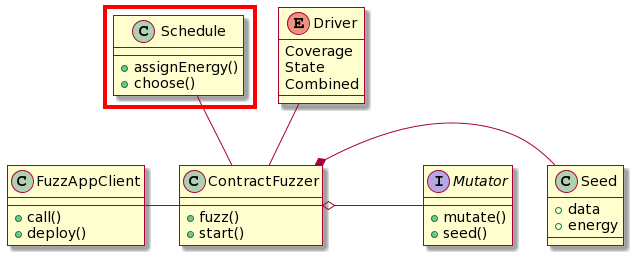
\includegraphics[width=0.85\textwidth]{figures/arc-schedule.png}
    \caption{AlgoFuzz architecture with schedule highlighted.}\label{fig:architecture-schedule}
\end{figure}

The schedule of AlgoFuzz is implemented through an exponential power schedule similar to the one proposed by AFLFast \cite{bohme_coverage-based_2016}.
This schedule assigns high energy to inputs that traverse paths or transitions that have been less frequently traversed.
How often a path or transition has been traversed is stored in dictionaries, one for the path frequency and one for the transition frequency.
Every time an input is executed the frequency of the path and transition that it traversed is incremented.
The keys of the dictionaries are the hashes of the paths and transitions.
As mentioned above, these frequencies are then used to first calculate the weighted frequency given the coefficient of the state.
The formula for the weighted frequency is the following:
\begin{figure}[htbp]
    \centering
    \[ w(s) = w_s * t(s) + w_c * p(s) \]
    \begin{tabular}{@{}>{$}l<{$}l@{}}
        s    & seed                                     \\
        w_s  & state weight                             \\
        w_c  & coverage weight (1 - $w_s$)              \\
        t(s) & frequency of transition traversed by $s$ \\
        p(s) & frequency of path traversed by $s$       \\
        w(s) & weighted frequency of $s$                \\
    \end{tabular}
\end{figure}

Then the energy is calculated with the following formula:

\begin{figure}[htbp]
    \centering
    \[e(s) = \dfrac{1}{w(s) ^ \alpha}\]
    \begin{tabular}{@{}>{$}l<{$}l@{}}
        %s      & seed                      \\
        %w(s)   & weighted frequency of $s$ \\
        \alpha & schedule exponent  \\
        e(s)   & energy of the seed \\
    \end{tabular}
\end{figure}

The schedule exponent is a parameter that can be configured for the schedule.
It determines by how much we prioritize less traversed paths and transitions.
For AlgoFuzz this value is hard coded to 5, this way we emphasize newer inputs more aggressively.
In the future, this could be a configurable value for the fuzzer or it could be dynamically changed during the fuzzing process.

After calculating the energy of each input, the schedule uses it to determine the probability of choosing an input.
The probability of an input being chosen is the normalized energy, which is calculated by dividing the energy of the input by the sum of all energies.

\section{Important Runtime information}
In this section, we will discuss the different metrics that we used to evaluate our fuzzer.

\paragraph{Number of calls executed} Shows us how efficient the fuzzer is at generating inputs and calling the application.
Since fuzzing is a random process, the number of calls executed needs to be very large to get meaningful inputs.

\paragraph{Number/Ratio of rejected calls} Any call that is rejected by the application is not interesting.
The ratio is the number of rejected calls divided by the total number of calls.
The lower the ratio, the better.
Fuzzers that have a low ratio of rejected calls have a higher probability of generating interesting inputs and finding the contract.

\paragraph{Number/Ratio of lines covered} The number of unique lines covered is the number of lines that were executed during the fuzzing process.
The ratio is the number of unique lines covered divided by the total number of lines in the \ac{TEAL} approval program of the contract.
This is a metric that is used by most fuzzers.

\paragraph{Number of unique paths} Every set of lines covered produced by a call is a coverage path.
This gives us a metric of how many different paths were executed during the fuzzing process.
In general, the more paths are covered, the better.
Although, a higher number of paths does not necessarily mean that more lines were covered.
This is because a path can be a subset of another path.

\paragraph{Number of unique state transition} We record all unique state transitions that were produced by the fuzzing process.
The more transitions are produced, the closer the fuzzer can be to finding a state that would invalidate the property test.

\section{Case Study: AlgoTether}
Before we go into the evaluation of our fuzzer, we will go through a case study of a smart contract that we wrote for this research.
The contract is called AlgoTether and it is a simple contract that allows users to mint and transfer tokens.
AlgoTether is translated from the Solidity contract of the Tether Token \cite{etherscanio_tether_nodate}, which is a stablecoin that is pegged to the US dollar.

The reason we decided to translate this contract is that there are no Algorand contracts that use the official \ac{ABI} and do not rely on box storage, which we do not support.
This makes it hard to find contracts that are long enough to be interesting for our evaluation.

\subsection*{Contract Features}
This contract represents an ERC20 token \cite{noauthor_erc-20_nodate}.
Each account has a balance of tokens that can be transferred to other accounts.
An account can also allow other accounts to spend tokens on its behalf.
In the Algorand version of the contract, we represent balances as local state in the account that owns the tokens.
For allowances, we store in the local state of the account that owns the tokens, a mapping from the account that is allowed to spend tokens to the amount of tokens that it is allowed to spend.
The key for the allowances is \texttt{allowance\_<spender>} where \texttt{spender} is the address of the account that is allowed to spend tokens.
Since we are using local state we need to declare it before deploying how much space we will need.
In our case, we will need only 3 local state values for the account, since we have at maximum 3 accounts.

The contract is \emph{ownable} which means there is an owner account that has special privileges and can perform certain operations that other accounts cannot.
The owner of the contract is the account that deployed the contract and it can be changed only by the current owner.

The contract is also \emph{pausable}, meaning that the owner can pause the contract, which will prevent any transfers from happening.

The contract also has a blacklist feature, which allows the owner to add accounts to a blacklist.
Accounts on the blacklist cannot transfer tokens.
The blacklisted accounts are stored on the global state of the contract, with the key \texttt{blacklist\_<acc>}.

\subsection*{Setup}
For this case study, we tried all the different combinations of drivers and fuzzers.
This gives us in total 6 different fuzzers: partial fuzzer with coverage driver, partial fuzzer with state driver, partial fuzzer with combined driver, total fuzzer with coverage driver, total fuzzer with state driver, and total fuzzer with combined driver.
We also tested the total and partial fuzzer with the combined driver using different state coefficients (or the weight of the state driver).
For this we used the weights from 0.1 to 0.9 with a step of 0.1.
The weights of 0 and 1 are not included since that would be almost the same as using coverage or state driver respectively.

The case study was conducted on a local machine with an Intel Core i7-8550U CPU and 16GB of RAM.
Each fuzzer was run 5 times with a timeout of 2 minutes.
The averages of the runs were gathered.

\subsection*{Results}
First we ran the experiment with the different coefficients to find out which one works best. We focused on two key questions:
\begin{itemize}
    \item Which coefficient leads to more state being covered?
    \item Which coefficient produces the most unique state transitions?
\end{itemize}

\begin{figure}[htbp]
    \centering
    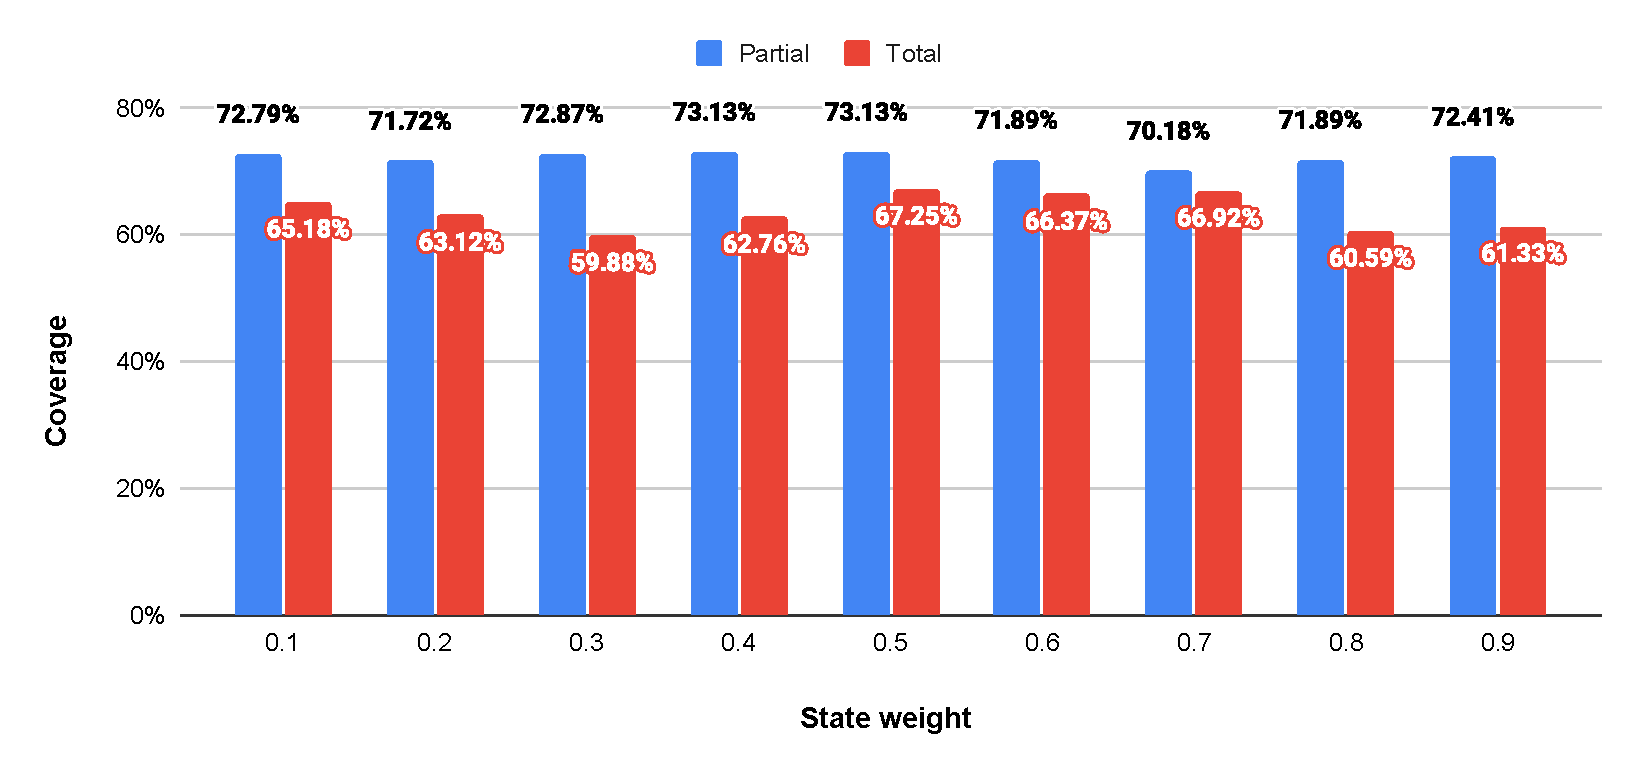
\includegraphics[width=0.9\textwidth]{charts/coef-cov-2.pdf}
    \caption{Coverage results with different coefficients.}\label{fig:case-study-coeff}
\end{figure}

To answer the first question we just looked at the percentage of lines covered which is shown in Figure \ref{fig:case-study-coeff}.
From which we can clearly see that the highest values are concentrated at the coefficient of 0.5.



For the second question we looked at the number of unique state transitions, which is shown in Figure \ref{fig:coef-trans}.
Here it is less clear which coefficient works best.
For the partial fuzzer, the number of transitions goes down as the state coefficient increases.
This seems counterintuitive at first, but it makes sense when see that the number of calls executed also goes down.
When we calculate the ratio of transitions to calls executed, we see that it is mostly staying the same throughout the different coefficients (at around 22\% for the partial fuzzer and 11\% for the total fuzzer).
In this case it is harder to say which coefficient works best, so we decided to use the coefficient of 0.5 based on the coverage results.

\begin{figure}[htbp]
    \centering
    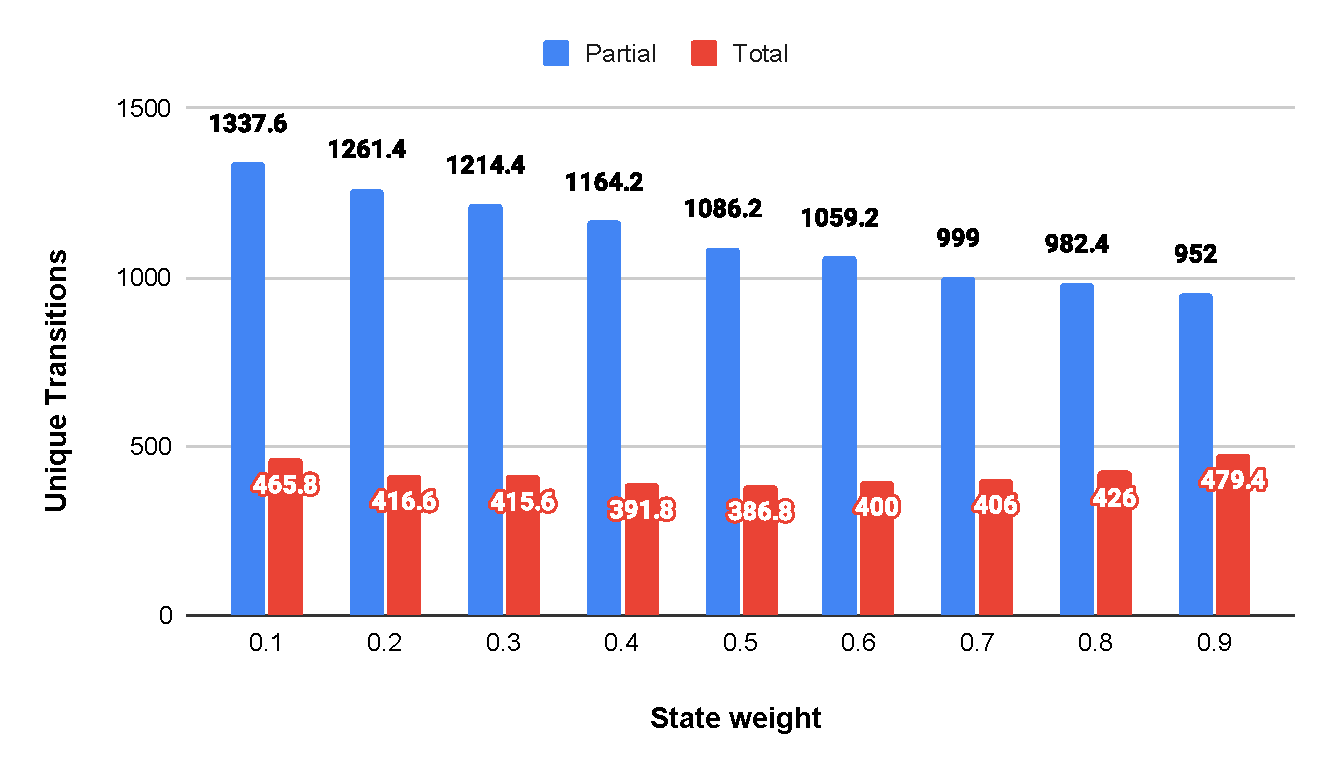
\includegraphics[width=0.9\textwidth]{charts/coef-trans-2.pdf}
    \caption{State transitions with different coefficients.}\label{fig:coef-trans}
\end{figure}

With the coefficients chosen, we ran the experiment again to compare the different fuzzers.
The results for rejected calls and coverage are shown in Figure \ref{fig:rej-cov}.

\begin{figure}[htbp]
    \centering
    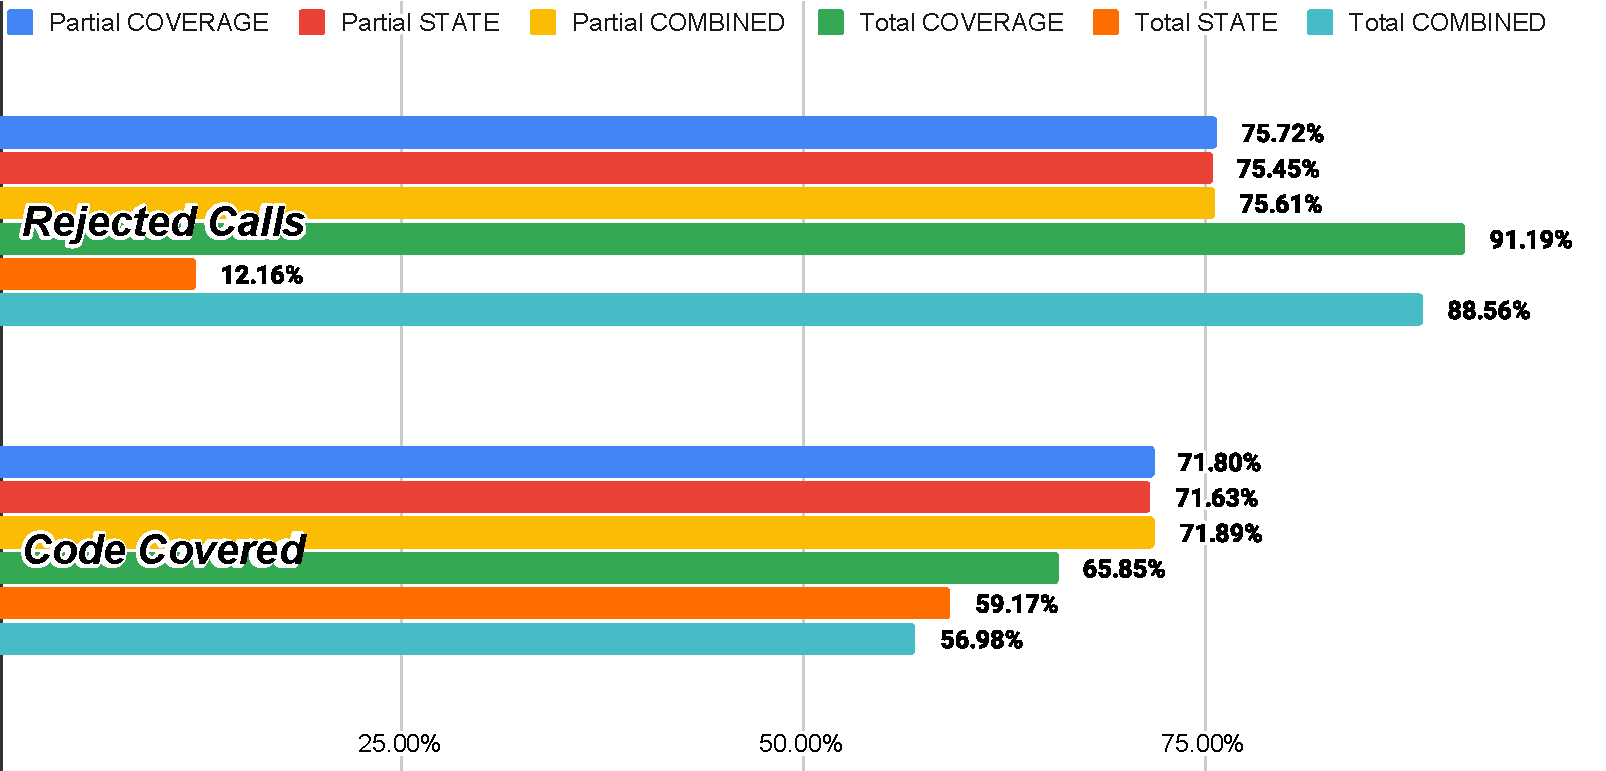
\includegraphics[width=0.8\textwidth]{charts/rej-cov.pdf}
    \caption{State transitions with different coefficients.}\label{fig:rej-cov}
\end{figure}

From the results we can see that the total fuzzer with the state driver has the lowest ratio of rejected calls by far.
This means that it is the most efficient at generating inputs that are accepted by the contract.
Aside from this, we can see that the partial fuzzer has higher coverage than the total fuzzer across all drivers.
And, as expected, for the total fuzzer the coverage driver has the highest coverage.

It was also interesting to see the amount of unique paths and state transitions that were covered by the different fuzzers, show


\begin{figure}[!htbp]
    \centering
    \subfloat[PyTeal][Unique Paths.]{
        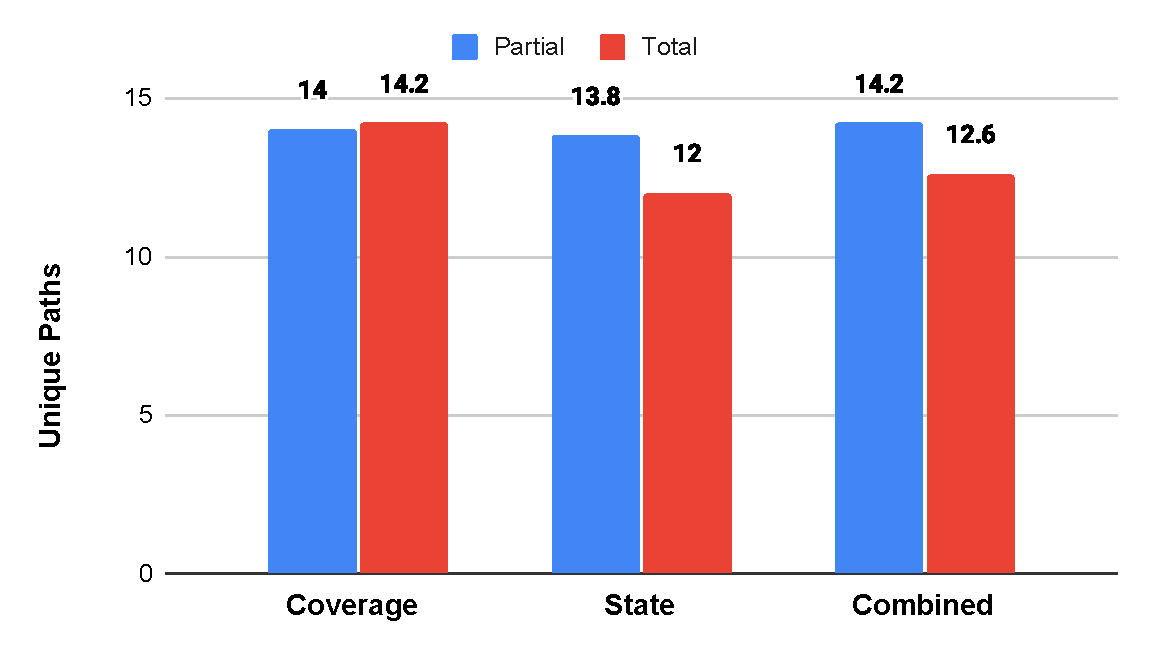
\includegraphics[width=0.47\textwidth]{charts/paths-2.pdf}
        \label{fig:paths}
    }
    \hfill
    \subfloat[TEAL][Unique Transitions.]{
        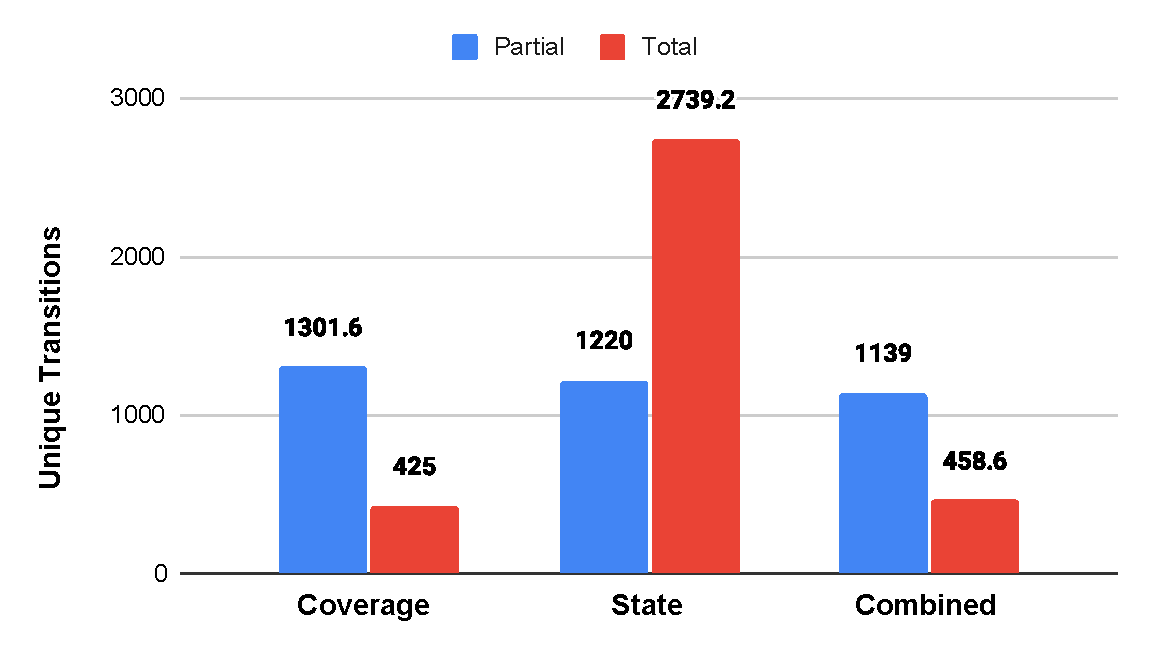
\includegraphics[width=0.47\textwidth]{charts/trans-2.pdf}
        \label{fig:trans}
    }
    \caption{Unique coverage paths and state transitions discovered.}
    \label{fig:path-trans}
\end{figure}

Different from the coverage results, the total fuzzer is not too far behind in terms of the amount of unique paths discovered.
For the state transitions, we see the partial fuzzer performs more or less the same regardless of the driver, at around 1200 transitions.
In contrast, the total fuzzer underperforms for the coverage and combined drivers at around 430 transitions.
The total fuzzer with the state driver show outstanding results with 2739.2 transitions discovered on average.
This goes hand in hand with the rejected calls results, since the state driver will most likely prioritize inputs which slightly change the state of the contract and therefore are safer.

From these results we can conclude that our fuzzer with the different configurations is able to cover a large amount of the code and state space of the contract.